%% LyX 2.0.4 created this file.  For more info, see http://www.lyx.org/.
%% Do not edit unless you really know what you are doing.
\documentclass[12pt,english]{report}
\usepackage{newcent}
\renewcommand{\familydefault}{\rmdefault}
\usepackage[T1]{fontenc}
\usepackage[utf8]{luainputenc}
\usepackage[a4paper]{geometry}
\geometry{verbose,tmargin=3cm,bmargin=3cm,lmargin=3.5cm,rmargin=2cm}
\pagestyle{empty}
\usepackage{babel}
\usepackage{verbatim}
\usepackage{float}
\usepackage{wrapfig}
\usepackage{graphicx}
\usepackage{setspace}
\usepackage{subscript}
\onehalfspacing
\usepackage[unicode=true,pdfusetitle,
 bookmarks=true,bookmarksnumbered=false,bookmarksopen=false,
 breaklinks=false,pdfborder={0 0 1},backref=false,colorlinks=false]
 {hyperref}

\makeatletter
%%%%%%%%%%%%%%%%%%%%%%%%%%%%%% Textclass specific LaTeX commands.
\newenvironment{lyxlist}[1]
{\begin{list}{}
{\settowidth{\labelwidth}{#1}
 \setlength{\leftmargin}{\labelwidth}
 \addtolength{\leftmargin}{\labelsep}
 \renewcommand{\makelabel}[1]{##1\hfil}}}
{\end{list}}

%%%%%%%%%%%%%%%%%%%%%%%%%%%%%% User specified LaTeX commands.
\usepackage{tocloft}
\usepackage{calc}
\usepackage{graphicx}
\usepackage[compact]{titlesec}
\usepackage[absolute]{textpos}
\usepackage[authoryear]{natbib}
\usepackage{titlesec}
\usepackage{caption}
\usepackage{url}

% for url breaks
\makeatletter
\g@addto@macro{\UrlBreaks}{\UrlOrds}
\makeatother

\def\UrlFont{\footnotesize\ttfamily}

% Important for page numbering
\pagestyle{plain}

% CHAPTER TITLE
% \titleformat command shape format label sep before after 
\titleformat
{\chapter}
[display]
{\normalfont}
{\large\raggedright\thechapter}{-24pt}
{\large\raggedleft}
[{\titlerule[1pt]}]

\titleformat{\section}
  {\normalfont\fontsize{14pt}{14pt}\selectfont\bfseries}{\thesection}{1em}{}

\titleformat{\subsection}
  {\normalfont\fontsize{12pt}{12pt}\selectfont\bfseries}{\thesubsection}{1em}{}

\titleformat{\subsubsection}
  {\normalfont\fontsize{11pt}{11pt}\selectfont\bfseries}{\thesubsubsection}{1em}{}



% Title margins
\titlespacing{\chapter}{0pt}{-3em}{3em}
\titlespacing{\section}{0pt}{3em}{0,5em}
\titlespacing{\subsection}{0pt}{2em}{0,5em}
\titlespacing{\subsubsection}{0pt}{1,5em}{0,5em}
\titlespacing{\paragraph}{0pt}{6pt}{6pt}


% figure caption
\captionsetup[figure]{font=small} 

\makeatother

\begin{document}
\begin{textblock*}{\paperwidth}(0mm,30mm)
\begin{center}  
\includegraphics[width=\paperwidth-400px]{graphics/logo} 
\end{center}
\end{textblock*}

\begin{textblock*}{\paperwidth}(30mm,235mm)
\noindent
SAE Berlin\\
Student Id: 18128\\
Course: AED412\\
Headinstructor: Boris Kummerer\\
Berlin, Germany 2012\\
Words: 5926
\end{textblock*}

\author{
by Karl Pannek
}

\title{\LARGE{Prototyping a Modular Analog Synthesizer}}
\maketitle{ }


\pagenumbering{arabic}
\setcounter{page}{2}
\renewcommand\cftpartdotsep{6.6} 
\renewcommand\cftchapdotsep{6.6} 


\chapter*{Table of Contents}

\renewcommand\contentsname{}
\vspace*{-8.5em} 
\tableofcontents


\chapter{Preface}


\section*{Introduction}

This paper constitutes an attempt to summarize the most important
facts and information on the topic of analog, modular synthesizers.
The range of discussed subjects involves a series of various perspectives,
including historical, theoretical, electronic and practical viewpoints. 

Its goal is to convey an understanding of the inner workings of electronic
synthesizers and their components. Moreover the reader is guided through
the process of creating a small but functional modular synthesizer
setup that is fun to play and experiment with. The intention was to
investigate the possibilities and limits in designing and building
an analog sound device for someone who had not been in contact with
analog synthesizers before, let alone building electronics devices.
The project was inspired by the film \emph{moog} (Fjellestad, 2004)
\nocite{Fjellestad:movie}\nocite{Fjellestad:movie}, a documentary
about Dr. Robert Moog, electronic instrument pioneer and inventor.


\section*{Chapter Overview}

The chapter \emph{Historic Evolution of the Synthesizer} represents
the research on the historical background of analog synthesizers since
the beginning of the twentieth century. It was tried to outline important
milestones in the historic development from the first electronic sound
generating devices until a point in time when manufacturers of modular
synthesizers have developed a profitable market.

Subsequently the most important concepts of subtractive synthesis
are summarized. A general overview over common sound generation and
processing methods is given, whereby all concepts are applicable to
both analog and digital synthesis. In chapter three these concepts
are taken one step further and discussed in the context of electronic
circuitry. Lastly the process of building an electronic synthesizer
prototype is described.


\chapter{Historic Evolution of the Synthesizer}


\section{Early Development Milestones}



Around 1900 american Thaddeus Cahill initiated a new era of music
by inventing a machine known as the Dynamophone or Thelharmonium \cite[p.~19]{Humpert1987}.
Working against incredible technical difficulties he succeeded to
create an electrical sound generator with a weight of around 200 metric
tons. It produced alternating sine wave shaped currents of different
audio frequencies. A modified electrical dynamo was used in conjunction
with several specially geared shafts and inductors to create the signals.
The Dynamophone could be played with a polyphonic keyboard and featured
special acoustic horns to convert the electrical vibrations into sound
\cite[p.~1]{Manning1985}. The timbre of the instrument was manually
shaped from fundamentals and overtones. This is known as the principle
of additive synthesis \cite[p.~730]{Bode1984}.

\begin{wrapfigure}{O}{4.5cm}%
\vspace*{-2em} 
\begin{center}

\includegraphics[width=4.5cm]{graphics/theremin}

\caption[
Leon Theremin performing the Aetherophone
\newline 
\url{http://www.npr.org/blogs/allsongs/2013/02/07/171385175/no-it-wasn-t-a-theremin-on-good-vibrations-remembering-paul-tanner
}]
{Leon Theremin performing the Aetherophone \label{fig-theremin}}
\end{center}
\vspace*{-2em} \end{wrapfigure}%


In 1924 the russian inventor Leon Theremin created the Aetherophone
(see figure \ref{fig-theremin}), which would later be known as the
Theremin. Unlike most electric instrument developed around that time,
the Theremin had no keyboard. It was played merely by hand motion
around two capacitive detecors, that generated electrical fields.
These were affected by the electric capacity of the human body. One
of these detectors was a vertical rod to control dynamics and the
other a horizontal loop to change the pitch \cite[p.~3]{Manning1985}.
``The theatricality of its playing technique and the uniqueness of
its sound made the Theremin the most radical musical instrument innovation
of the early 20th century.'' \cite[p.~6]{Dunn1992}

Some organ-like precursors to the synthesizer were the Ondes Martenot
and the Trautonium, which were devised just a few years later. The
Ondes Martenot is one of the few early electric instruments, that
are still in concert- and theatre use in their original design today
\cite[p.~20]{Humpert1987}.

The Givelet (1929) was a commercially more successful instrument,
since it was designed as a cheap alternative to pipe organs. These
instruments were polyphonic and unified the concepts of the Pianola
- a self-playing piano, controlled by pre-punched tape - with electronic
sound genaration. The ability to program electronic sounds should
lead the way for future devices such as the RCA synthesizer or computer
music production in general. However, the Givelet was about to take
a back seat, when Laurens Hammond published his Hammond Organ in 1935.
Its technical operation principle is reminiscent of the Dynamophone,
since it also involved rotating discs in a magnetic field \cite[p.~3]{Manning1985}.

\begin{wrapfigure}{O}{4.5cm}%
\vspace*{-2em} 
\begin{center}

\includegraphics[width=4.5cm]{graphics/bode-melochord}


\caption[
Harald Bode tuning his first Melochord
\newline 
\url{http://cec.sonus.ca/econtact/13_4/bode_history.html}]
{Harald Bode tuning his first Melochord \label{fig-bode}}
\end{center}
\vspace*{-2em} \end{wrapfigure}%
The german engineer Harald Bode contributed to the design of several
new instruments from the 1930's on, like the warbo formant organ (1937)
or later the Melochord (1949) (see figure \ref{fig-bode}). He was
primarily interested in providing tools for a wide range of musicians,
which is why his contributions straddled between the two major design
traditions of new sounds versus imitation of traditional ones. He
turned out to be one of the central figures in the history of electronic
music, since he was also one of the primary technicians in establishing
the classic tape music studio in Europe \cite[p.~9]{Dunn1992}.

Bode was one of the first engineers to grasp the significance of the
invention of the solid state transistor for sound synthesis. In an
article published in 1961 he draws particular attention to the advanteges
of modular design. ``The versatility of transistor-based electronics
made it possible to design any number of devices which could be controlled
by a common set of voltage characteristics.'' \cite[p.~117]{Manning1985}.
But it was not until the early 1960's that major advances in electronic
design took shape \cite[p.~19]{Dunn1992}.


\section{The First Synthesizers}

In 1955 the laboratories of the Radio Corporation of America (RCA)
introduced a new and very advanced machine to the public named the
Olson-Belar Sound Synthesizer, later known as the RCA Mark I Music
Synthesizer. It combined many means of tone generation and sound modification
known at the time and is considered the first synthesizer. Mark I
was built with the specific intention of imitating traditional instrument
sounds and to reduce the costs of the production of popular music
by replacing musicians. However, the machine proved unsuitable for
its original intent and was later used completely for electronic music
experimentation and composition \cite[p.~15-16]{Dunn1992}. The synthesizer
could not be played in the conventional sense in real time. Instead
musical information had to be pre programmed as punched holes in a
large paper tape. Harry Olson and Herbert Belar produced an improved
Mark II Synthesizer in 1957, which the nickname \emph{Victor} was
given.

Around the same time the outstanding guitarist and inventor Les Paul
became famous with his multitrack guitar recordings. He stimulated
many innovators not only with the success of his multitrack recorder,
but also with his methods of electronic sound processing. Harald Bode
was so impressed and inspired by his work, that he built a system
consisting of a number of electronic modules for sound modification
in late 1959 through 1960. His system featured ring modulator devices,
envelope followers and generators, voltage-controlled amplifiers,
filters and other \cite[p.~733]{Bode1984}. The modular concept of
his device had proven attractive due to its versatility and predicted
the more powerful modular synthesizers that emerged in the early 1960's
\cite[p.~20]{Dunn1992}. 

In 1963 Robert Moog, a passionate inventor from Ithaca, New York,
United States, was selling kits of transistorized Theremins \cite[p.~20]{Dunn1992}.
In the documenteray \emph{moog} (Fjellestad, 2004) he states that
he had been completely obsessed with building and later designing
Theremins since the age of 14. A year later he built a transistor
based voltage-controlled oscillator and amplifier for the composer
Herbert Deutsch. This led Moog to the presentation of a paper entitled
\emph{Voltage-Controlled Electronic Music Modules} at the sixteenth
annual convention of the Audio Engineering Society, which had stimulated
widespread interest \cite[p.~117-118]{Manning1985}. 

\begin{wrapfigure}{I}{5cm}%
\vspace*{-2em} 
\begin{center}

\includegraphics[width=5cm]{graphics/buchla}

\caption[
Donald Buchla with a Series 100 system in the 1960's
\newline 
\url{http://www.soundonsound.com/sos/dec05/articles/buchla200e.htm}]
{Donald Buchla with a Series 100 system in the 1960's \label{fig-buchla}}
\end{center}
\vspace*{-3em} \end{wrapfigure}%
 Similar developments had been taking place at the west coast of the
united states. Morton Subotnick and Ramon Sender started their career
in electronic music experimentation and became increasingly dissatisfied
with the severe limitations of traditional equipment at the San Francisco
Tape Music Center. They sought out to hire a competent engineer and
met Donald Buchla (see figure \ref{fig-buchla}) \cite[p.~117-118]{Manning1985}.
Their discussions resulted in the concept of a modular voltage-controlled
system. Buchla's design approach differed significantly from Moog.
He rejected the idea of a synthesizing familiar sounds and resisted
the word \emph{synthesizer} ever since. To him it seemed much more
interesting to emphasize new timbral possibilities and stress the
complexity that could arise from randomness. At the same time Buchla
was fascinated with designing control devices other than the standard
keyboard, which Moog decided to use for playing \cite[p.~20]{Dunn1992}.
``Buchla has maintained his unique design philosophy over the years
producing a series of highly advanced instruments often incorporating
hybrid digital circuitry and unique control interfaces.'' \cite[p.~23]{Dunn1992}

\begin{wrapfigure}{O}{5cm}%
\vspace*{-2em} 
\begin{center}

\includegraphics[width=5cm]{graphics/switched-on-bach}

\caption[
Switched-On Bach LP artwork
\newline 
\url{http://www.wendycarlos.com/discs.html}]
{Switched-On Bach LP artwork \label{fig-switched}}

\end{center}
\vspace*{-2em} \end{wrapfigure}%
 In 1966 Robert Moog's first production model was available from the
business R.A. Moog Co. that he had founded \cite[p.~20]{Dunn1992}.
At this time Walter Carlos, an audio engineer from New York who advised
Robert Moog while perfecting his system, worked with Benjamin Folkman
to produce an album of titles by Johann Sebastian Bach interpreted
only with Moog synthesizers (see figure \ref{fig-switched}). With
the title \emph{Switched-on Bach} they demonstrated the performance
of the system so convincingly, that they hit the pop music charts
and sold a million LP's \cite[p.~45]{Ruschkowski1990}. 

By the end of the decade two other manufacturers entered the market:
ARP in America and EMS Ltd. in England. They had become major rivals
for Moog and Buchla. Synthesizer production was dominated by these
four companies for several years, whereby each firm struggled for
a major share of a highly lucrative, rapidly expanding market \cite[p.~118]{Manning1985}.


\chapter{Theory of Subtractive Synthesis}

During the last century different kinds of synthesis methods have
emerged. The subtractive synthesis however, appears to be the most
common one. It is a method of sound synthesis, where partials of the
initially generated signal are attenuated with a filter to change
the timbre of the sound. But how can these sounds actually be synthesized?
And what exactly does a filter do? These questions will be examined
in the following.


\section{Sources}

Acoustic events can generally be divided in two groups: noises and
tones. Whereas tones - as opposed to noise - are classified as sound
waves, that have determined set of frequencies, which oscillate in
a sinoidal manner. However this is only a theoretical classification,
since most natural sounds are a combination of the two \cite[p.~52]{Ruschkowski1990}. 


\subsection{Wave Oscillation}

\begin{wrapfigure}{O}{4.5cm}%
\vspace*{-2em} 
\begin{center}

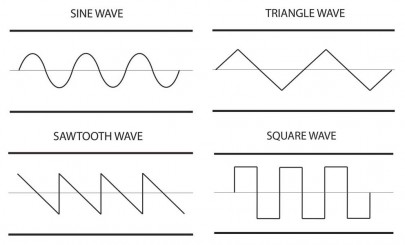
\includegraphics[width=4.5cm]{graphics/waveforms}

\caption[
Common oscillator waveforms
\newline 
\protect{\cite[p.~49, edited by author]{Anwander2011}}]
{Common \linebreak oscillator waveforms \label{fig-waves}}
\end{center}
\vspace*{-2em} \end{wrapfigure}%
At the root of every artificial tone generating system there is an
element that produces an oscillation. This element is mostly described
as the oscillator, which represents the very source of what can be
heard eventually. The oscillator produces a wave, that moves between
an amplitude-minima and -maxima. Its waveform (shape of the wave)
determines the overtone structure and therefore the timbre of this
basic source sound. Oscillators often provide several waveforms between
which it is possible to switch back and forth (see figure \ref{fig-waves}).
The pitch of the output signal is defined by the frequency of the
wave and must oscillate between 20 Hz and 20 kHz in order for it to
be audible to humans \cite[p.~124]{Friesecke2007}. The output signal
can later be processed and modulated in several ways.

Oscillators that swing at an infrasonic frequency - meaning a frequency
so low, that it is not hearable anymore - are called low frequency
oscillators (LFO). They are used to control parameters of different
components of the synthesizer periodically. For example to influence
the pitch of another oscillator to get a vibrato - or the amplitude
to get a tremolo effect. Some oscillators frequencies range from very
low to very high, in which case a distinction between oscillator and
LFO is unnecessary.


\subsubsection{Characteristics of Common Waveforms}
\begin{lyxlist}{00.00.0000}
\item [{Sine}] The most basic waveform is the sine wave. It contains no
overtones at all and sounds round and dull.
\item [{Sawtooth}] The sawtooth, also known as saw or ramp waveform sounds
very bright, sometimes described as trumpet-like \cite[p.~49]{Anwander2011}.
It consist of a complete series of harmonics and is therefore well
suited for subtractive synthesis. There are two types of sawtooth
waves: rising and descending. 
\item [{Triangle}] Composed of only odd harmonics, the triangle wave has
a much softer, flute-like sound.
\item [{Square}] Also known as rectangle, the square wave also consists
of odd harmonics only, but the level distribution of its harmonics
is different. Its timbre reminds of woodwind instruments \cite[p.~55]{Ruschkowski1990}.
A true square wave has a 50 \% duty cycle - equal high and low periods.
However, oscillators often feature a pulse width parameter, trough
which the high-low time ratio can be accessed. This has a distinct
influence on the wave's timbre. In this case, the square becomes a
pulse waveform. 
\end{lyxlist}

\subsection{Noise Generation}

A different approach on the creation of source audio material is resembled
by noise generators. ``In very loose terms, noise is a complex waveform
with components of every frequency, each attaining a completely random
amplitude at any give instant.'' \cite[p.~1]{Henry2009}


\subsubsection{Noise Types}
\begin{lyxlist}{00.00.0000}
\item [{White}] Equal power density in any band of the frequency spectrum
\item [{Pink}] Power density decreases by 3dB per octave; also referred
to as 1/f noise
\item [{Brown}] Power density decreases by 6dB per octave; also referred
to as 1/f\textsuperscript{2}noise
\end{lyxlist}
The names of these noise types were derived from the spectral distribution
of the correspondingly colored light \cite[p.~155]{Friesecke2007}.


\subsection{Triggering Notes}

In order to use the previously discussed signal generators in a musical
context, it is necessary to cut off their stationary signals when
no note is being played. This is accomplished by routing the output
signal of the generator to an amplifier and providing it with a gate
signal. The source of the gate signal can be a keyboard or a sequencer,
which would also send a pitch value to the oscillator to set its frequency
\cite[p.~36]{Anwander2011}.


\section{Signal Processing}

In their raw shape the mentioned source signals sound rather underwhelming,
since they produce fixed timbres lacking of distinctive qualities
\cite[p.~49]{Manning1985}. To get a more interesting sound, the signal
can be manipulated in acoustic color or dynamics by one or more processing
units.


\subsection{Dynamic Envelopes}

The most important component responsible for shaping the dynamic structure
of a note is the envelope. It is triggered by the gate on/off signal
and outputs a control signal that fades between the different state
phases of a note. The rapidity of these changes is adjusted by parameters,
that represent these states. Its output signal can be used to control
an amplifier and therefore shape the dynamic structure of the note.
The most common envelope type is the ADSR, which stands for attack,
decay, sustain, release. 
\begin{lyxlist}{00.00.0000}
\item [{Attack}] Sets how long the envelope signal rises after a note was
triggered
\item [{Decay}] Sets how long it takes for the envelope signal to drop
from its maximum to the sustain level after the attack phase was completed
\item [{Sustain}] Sets the output level for the time period after the decay
phase and before the gate signal was terminated
\item [{Release}] Sets the length of the fade out after the note has ended
\end{lyxlist}
Envelopes can also be used to control other parameters, for example
the cutoff frequency of a filter (see chapter \ref{sub:filters}). 


\subsection{Filtering \label{sub:filters}}

The filter is the processing component responsible for the sound changes,
that people associate with \emph{the typical synthesizer sound} \cite[p.~53]{Anwander2011}.
They remove a spectrum of frequencies from their input signal above
or below the cutoff frequency and are often used in conjunction with
an envelope or LFO modulation on the cutoff. This cutoff frequency
is an important parameter determining the frequency at which the signal
begins to be attenuated. The slope of the filter determines how abrupt
frequencies are being cut. Another common parameter is called resonance.
It controls the level of a feedback loop, emphasizing the timbre at
the cutoff frequency.

Filters can generally be divided into two categories: Low pass and
high pass (also called high cut and low cut). To get a band pass,
low- and high pass are connected in series. When connected in parallel,
they become a band stop or band reject filter. Lastly the all pass
filter should be mentioned, which does not change the frequency spectrum
but merely influences the phase of the signal around its cutoff \cite[p.~55]{Anwander2011}. 


\section{Controllers}

Controllers can be characterized by the way of how humans interact
with them and how their output signal is applied in controlling other
components of the system \cite[Ch.~1A, p.~5]{Hutchins1975}. A keyboard
for example is a manual controller, since it is the movement of the
players fingers which are translated into a voltage or control value
and then used to control pitch and amplitude of a note. The same applies
for rotary knobs and faders or touch sensitive surfaces. 

Sequencers on the other hand are programmable controllers. They are
not dependent upon a manual interaction except for their programming
and activation. 


\section{The Modular Approach}

A modular synthesizer is an instrument, where sound generators, processors
and control facilities are presented in separate independent entities
called modules. These modules are not wired in a preconceived way,
but are connected with patch chords. The second essential aspect is
the concept of inter-modular controllability, with which modules may
modulate or regulate other modules. 


\chapter{Analog Synthesis}

The previously discussed theoretical concepts can generally be applied
to both analog and digital synthesizers. In this chapter some of these
concepts are transferred into the electronic context.


\section{General}

In digital synthesis audio signals and control signals are often being
differentiated. This is because computing power can be saved by limiting
the sample rate for control signals, since they usually only require
a fraction of the amount of sampling values to get acceptable results.

In the area of analog modular synthesis it is important to know that
signals are nothing but alternating and/or direct currents usually
with voltages ranging from -5 to +5 volts. That is why there is no
difference between audio and control signals. This has a great impact
on the extend of possibilities especially in modular systems. One
of the consequences is that an oscillator can control the frequency
of a second oscillator with its output signal. This is known as frequency-modulation
or FM synthesis.

However, when combining or mixing control and audio signals one should
be aware of the following phrase, stated by Donald Buchla: ``DC offset
doesn't make any difference in the sound domain but it makes a big
difference in the structural domain, whereas harmonic distortion makes
very little difference in the control area but it can be very significant
in the audio areas.'' \cite[p.~23]{Dunn1992}


\section{Modules}

In a modular synthesizer setup, all sound generating and processing
modules are aggregated and connected to a central power supply with
a common ground. Among the modular components the signals are transferred
via patch chords. The modules should be engineered to have the lowest
possible output impedance and a relatively high input impedance. A
common impedance ratio is 1:100. 

Below, the basic circuitry principles of some essential synthesizer
components will be examined.


\subsection{Oscillator \label{sub:electronic-oscillator}}


\subsubsection{Natural Resonance }

The most simple form of an oscillator circuit producing a sawtooth
signal can be realized with just a few parts (see figure \ref{fig-sawosc}).
A current charges a capacitor at a certain rate. Between the electrodes
of the capacitor a voltage potential rises. Meanwhile the voltage
is constantly compared with a reference voltage by a detector (Schmitt
trigger). Once it reaches the predefined threshold, an electronic
switch (transistor) is activated. This switch short-circuits the capacitor
and discharges it, causing the output voltage to drop back to its
initial potential. This is happening continuously, whereas the rate
of the repetition determines the frequency of the generated signal. 

\begin{figure}[H]
\begin{center}

\includegraphics[width=0.8\textwidth]{graphics/sawtooth-oscillator-circuit}

\caption[
Abstract circuit scheme of a basic sawtooth oscillator
\newline 
\protect{\cite[Ch. 5B, p. 3]{Hutchins1975}}]
{Abstract circuit scheme of a basic sawtooth oscillator \label{fig-sawosc}}
\end{center}
\end{figure}


To get a triangle shaped output signal, the current source can be
reversed in response to the detector (see figure \ref{fig-triosc})
\cite[Ch.~5B, p.~3]{Hutchins1975}.

\begin{figure}[H]
\begin{center}

\includegraphics[width=0.8\textwidth]{graphics/triangle-oscillator-circuit}

\caption[
Circuit scheme of a simple triangle oscillator
\newline 
\protect{\cite[Ch. 5B, p. 3]{Hutchins1975}}]
{Circuit scheme of a simple triangle oscillator \label{fig-triosc}}
\end{center}
\end{figure}


\pagebreak

These two waveforms can be wave-shaped into to other common basic
waveforms. All required wave shaping methods are fairly simple and
their accuracy is sufficient for musical purposes. The sine wave is
an exception, because there is no simple electronic method of creating
a pure sine wave. What is generally used is a rounded triangle, which
gives at least 1 \% of harmonic distortion. To get a purer sine wave,
the harmonics can be filtered out with a voltage-controlled filter
following in the signal chain \cite[Ch.~5B, p.~3-4]{Hutchins1975}.


\subsubsection{Voltage Control}

How fast the capacitor is charged is determined by the intensity of
the current that it is being charged with. This current is being extracted
from a voltage, which of course can be a control voltage.

However, creating a stable voltage-controlled oscillator design presents
one of the toughest challenges for musical engineers, because the
human ear is extremely sensitive to pitch changes. Also compositional
processes like multitrack recording plainly reveal errors in pitch
relationships \cite[Ch.~5B, p.~1]{Hutchins1975}. The voltage to pitch
distribution curve of an oscillator is determined by its exponential
response to the voltage at its CV input. In a volt per octave system
an increase by 1 volt at the input must result in a doubling of the
oscillation frequency at the output. Thus octave purity is achieved. 

A major issue that oscillator designers have to face are temperature
influenced variations of the electrical parameters of the system,
causing the oscillator pitch to drift when temperature changes occur.
To overcome this problem some kind of temperature compensation should
be implemented.


\subsection{Filter \label{sub:electronic-filter}}


\subsubsection{Passive Filter}

Filter circuits are generally based upon the fact that the transfer
of alternating currents through a capacitor becomes increasingly weak
below a certain frequency. A signal simply passed through a capacitor
resembles a high pass filter. If the capacitor is connected to the
ground the high frequencies are short circuited and low frequencies
remain in the signal path. To control the charging time of the capacitor
and therefore the cutoff frequency a resistor is added. This is referred
to as a resistor-capacitor (RC) element. This simple circuit represents
a passive, first-order filter with a roll-off of 6 dB per octave.
To increase the slope of the filter multiple RC elements can be connected
in series \cite[p.~57]{Anwander2011}. 

\pagebreak

Nevertheless this poses some disadvantages, because the filter stages
influence each other. The resistor of the first filter affects the
resistance of the second. This can be dealt with by designing the
second filter to have a much higher impedance. Unfortunately a high
impedance circuit is much more prone to interferences and signal noise
\cite[p.~97]{Sontheimer2004}.


\subsubsection{Active Filter}

\begin{wrapfigure}{O}{5.5cm}%
\vspace*{-2em} 
\begin{center}

\includegraphics[width=5.5cm]{graphics/Sallen-Key-Filter-Lowpass}

\caption[
Active Sallen-Key low pass filter circuit scheme
\newline 
\url{http://de.wikipedia.org/wiki/Sallen-Key-Filter}]
{Active Sallen-Key low pass filter circuit scheme \label{fig-sallenkey}}
\end{center}
\vspace*{-2em} \end{wrapfigure}%
 A better and more flexible solution is the usage of an active filter
design, like the Sallen-Key filter (see figure \ref{fig-sallenkey}).
This is a common second-order filter, which is applicable as a low
or high pass, whereby only resistors and capacitors have to be swapped
\cite[p.~97]{Sontheimer2004}. Resistor (R\textsubscript{2}) and
capacitor (C\textsubscript{2}) can be identified to form a low pass
section \cite[Ch.~4B, p.~4]{Hutchins1975}. 

To be able to change the cutoff frequency via voltage control the
frequency defining resistor could be replaced with a voltage controlled
resistor \cite[p.~198]{Lancaster1975}.


\subsection{Envelope Generator}

\begin{wrapfigure}{O}{7cm}%
\vspace*{-2em} 
\begin{center}

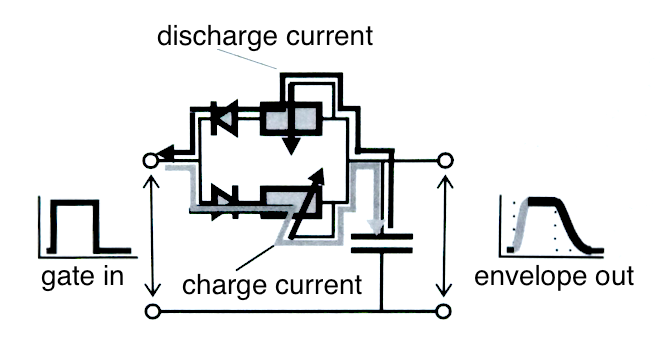
\includegraphics[width=7cm]{graphics/envelope3}

\caption[
Principle circuit diagram of an AR envelope 
\newline 
\protect{\cite[p.~41, edited by author]{Anwander2011}}]
{Principle circuit diagram of an AR envelope \label{AR-envelope}}


\end{center}
\vspace*{-2em} \end{wrapfigure}%
 The envelope generator is based on the principle of slew-rate limiting.
The rapid changes in the level of the gate voltage can be decelerated
by again using a resistor-capacitor element. By using a potentiometer
in the place of the resistor the charging time and therefore the speed
of the voltage alteration can be adjusted. To get a typical attack-release
(AR) envelope the charge and discharge times should be adjusted separately.
To achieve this two preceding potentiometers with a diode each should
be connected. The diodes must be pointed in opposite directions (see
figure \ref{AR-envelope}). 


\chapter{Building a Modular Synthesizer}


\section{Introduction \label{sec:building-introduction}}

It is relatively easy to find circuits to construct simple oscillators
and filters based on the fairly comprehensible concepts of resonant
circuits and RC elements (see chapter \ref{sub:electronic-oscillator}
and \ref{sub:electronic-filter}). However, as their flexibility and
capabilities increase (e.g. controlling the frequency of an oscillator
with 1 volt per octave), the circuits tend to get exceedingly complex,
requiring solid expertise in electronics.

This is why it was decided to switch to the usage of pre-designed,
professionally manufactured circuit boards for this project as opposed
to elaborating all the circuits on perfboards as originally intended.
This made the goal of intermodular controllability attainable more
easyily. The downside of this approach are higher costs for boards
and parts. However, the quality of the end-product is impressing.
Also the time saving using this strategy is not to be underestimated.

During the research phase of this project it came to the authors attention,
that a modular synthesizer building workshop would be taking place
in Berlin monthly. It is organized by a spanish collective from barcelona
called \emph{befaco} (\url{http://befaco.org}). At the workshop it
is possible to acquire various module kits containing all necessary
parts and also receive tips and support while assembling them. 

Due to budget limitations, it was tried to arrange a smaller setup
that would still offer lots of sound design possibilities.


\section{Formats and Interfaces}

There are several formats for module sizes, power supply plugs or
patch chord connectors which emerged out of the production lines of
various module manufacturers. For example Doepfer's modules are only
compatible with their EuroRack cases, with a height of 128.5mm. These
EuroRack modules use jack connectors for patching. In the DIY modular
synth scene it is a common practice to use banana jack connectors
instead of mini jack for patching. Those have the possibility of stacking
the connectors on top of each other and split the signal without having
to use a multiplier module. In this project the modules are EuroRack
size, but use banana plugs. 


\section{Building}

To get started with building electronic equipment, one has to obtain
some tools first. This includes a soldering iron - best with adjustable
temperature, a role of quality soldering tin, a desoldering pump and
pliers for cutting and bending wire. 

Soldering is a process of mounting electronic parts onto a circuit
board by heating up board and component and then melting the soldering
tin into the joint. A good temperature for the soldering iron is between
300° and 350° celsius. The iron should not be pressed onto the joint
for too long, because there is a risk of destroying the component
if it is sensitive to heat.


\section{Power Supply and Case}

For the power unit a universal power supply circuit was chosen from
Robert Sontheimers audio circuit technology book \cite[p.~74]{Sontheimer2004}
and mounted onto a perfboard. Instead of the 7815 and 7915 voltage
regulator ICs the 7812 and 7912 were used in order to get a +/-12
volt power supply with a center tap for the ground. The modules can
be connected to the four male 16-pin flat ribbon connectors, that
were added to make the power supply compliant to the EuroRack standard.
Another possibility would be to make a flying bus board by attaching
those connectors to a flat ribbon cable that lies in the case. Or
even just fix female connectors to the cable and plug them directly
into the modules. Additionally it is planned to add an IEC socket
and a power switch for comfortable on and off switching and more steady
starting current.

The case is a simple rack constructed from a few pieces of wood that
are held together by 19 inch rails equipped with thread rails to fasten
the modules.

\pagebreak


\section{Front Panels}

\begin{wrapfigure}{R}{0.22\textwidth}%
\vspace*{-2.5em} 
\begin{center}

\includegraphics[scale=0.6]{graphics/output-module-panel}

\caption[
Output module template 
\newline
\url{http://befaco.org}
]
{Output module template \label{fig-frontpanel}}

\end{center}
\vspace*{-2em} \end{wrapfigure}%
 

The panels for all modules were made from pre-cut aluminum plates
with a white varnish. The labels for knobs and banana sockets are
printed on the plates with a method, that is similar to homemade circuit
board etching%
\footnote{For etching the template would be transferred onto a copper board
and put into an acid bath.%
}. A mirror-inverted label template (see figure \ref{fig-frontpanel})
is printed onto a piece of high gloss paper for inkjet printers -
but with a laser printer. It is cut and placed face down onto the
upper side of the panel. By thoroughly pressing down a hot flat iron
(for ironing clothes) onto the panel for a few minutes, the toner
cartridge particles move to the panel. The paper residues need to
be removed by placing the panel in some water and rubbing them off
with a sponge. Afterwards the panel is sealed with transparent lacquer.
Once the panel is dried, the holes for the knobs, switches, etc. can
be prepunched and drilled. Lastly all boreholes are deburred. 

\vspace*{-0.5em} 


\section{BF-22 Filter }

\begin{wrapfigure}{R}{0.36\textwidth}%
\vspace*{-2.5em} 
\begin{center}

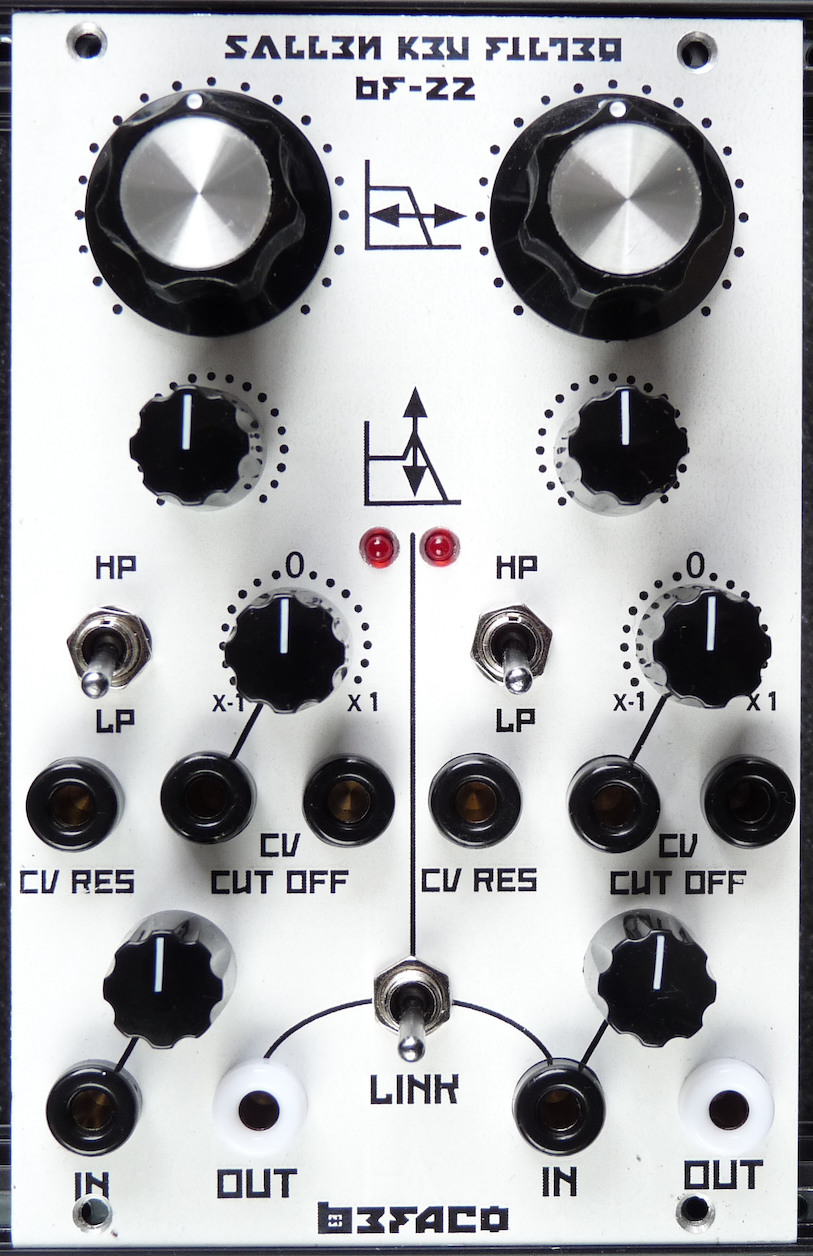
\includegraphics[width=0.36\textwidth]{graphics/bf22-2}

\caption{BF-22 filter module \label{bf22front} }



\end{center}
\vspace*{-2em} \end{wrapfigure}%


This module (shown in figure \ref{bf22front}) is an extended copy
of the filter from the legendary Korg MS-20 and is based upon the
principle of the Sallen-Key filter (see chapter \ref{sub:electronic-filter}).
It combines two linkable filter stages in one module. Each stage features
cutoff and resonance knobs and the corresponding CV inputs, whereas
the cutoff frequency input can be attenuated and inverted with one
knob representing modulation depth (labeled: X-1 ... 0 ... X1). The
HP/LP switch determines, if the filter is used in high pass or low
pass mode. 

When turning resonance up, at one point the filter begins to self-resonate
at the given cutoff frequency, which means that the filter can also
be utilized as an oscillator.

\vspace*{1.5em} 

\begin{wrapfigure}{R}{0.36\textwidth}%
\vspace*{-1em} 
\begin{center}

\includegraphics[width=0.36\textwidth]{graphics/bf22-board}

\caption{BF-22 main circuit board \label{bf22board}}


\end{center}
\vspace*{-2em} \end{wrapfigure}%
 Therefore a volt per octave input for the cutoff control voltage
was added, to be able to control the oscillating frequency in a musical
context. 

A look at the oscilloscope shows a sine like waveform. Turning the
resonance to the maximum, the filter goes into distortion and the
wave becomes more square causing the sound to get more rough. The
amount of distortion is visually represented by a red LED. 

Below the front panel sits an interface board where the knobs, switches,
LEDs and banana sockets are mounted to. A thirty pin socket connects
the interface board to the main circuit board (see figure \ref{bf22board}),
which contains the signal processing circuitry. The socket for the
power supply sits on the very bottom.

\begin{comment}
Will we get a complete schema somewhere in the appendix or something?
The description is nice to read but I'm quite sure one could not replicate
your prototype from this text alone.
\end{comment}



\section{Output}

The output module is responsible for transforming the \emph{hot}%
\footnote{The term hot signal is used commonly to describe signals with a relatively
high voltage.%
} synthesizer signal to a standard line level. It can be used in a
dual mono mode, picking up two separate output signals from tip and
ring of the 6.35 mm output jack. The mono switch splits the signal
to tip and ring. The phones output provides the output signal optimized
for headphones.

Additionally the module features a switch which activates a high pass
filter. The idea is to be able to protect speaker systems from high
energy bass signals. In the lower section 3 banana to jack patch sockets
were added.

\vspace*{1.5em} 

\pagebreak


\section{MIDI Input}

\begin{wrapfigure}{R}{0.36\textwidth}%
\vspace*{-3em} 
\begin{center}

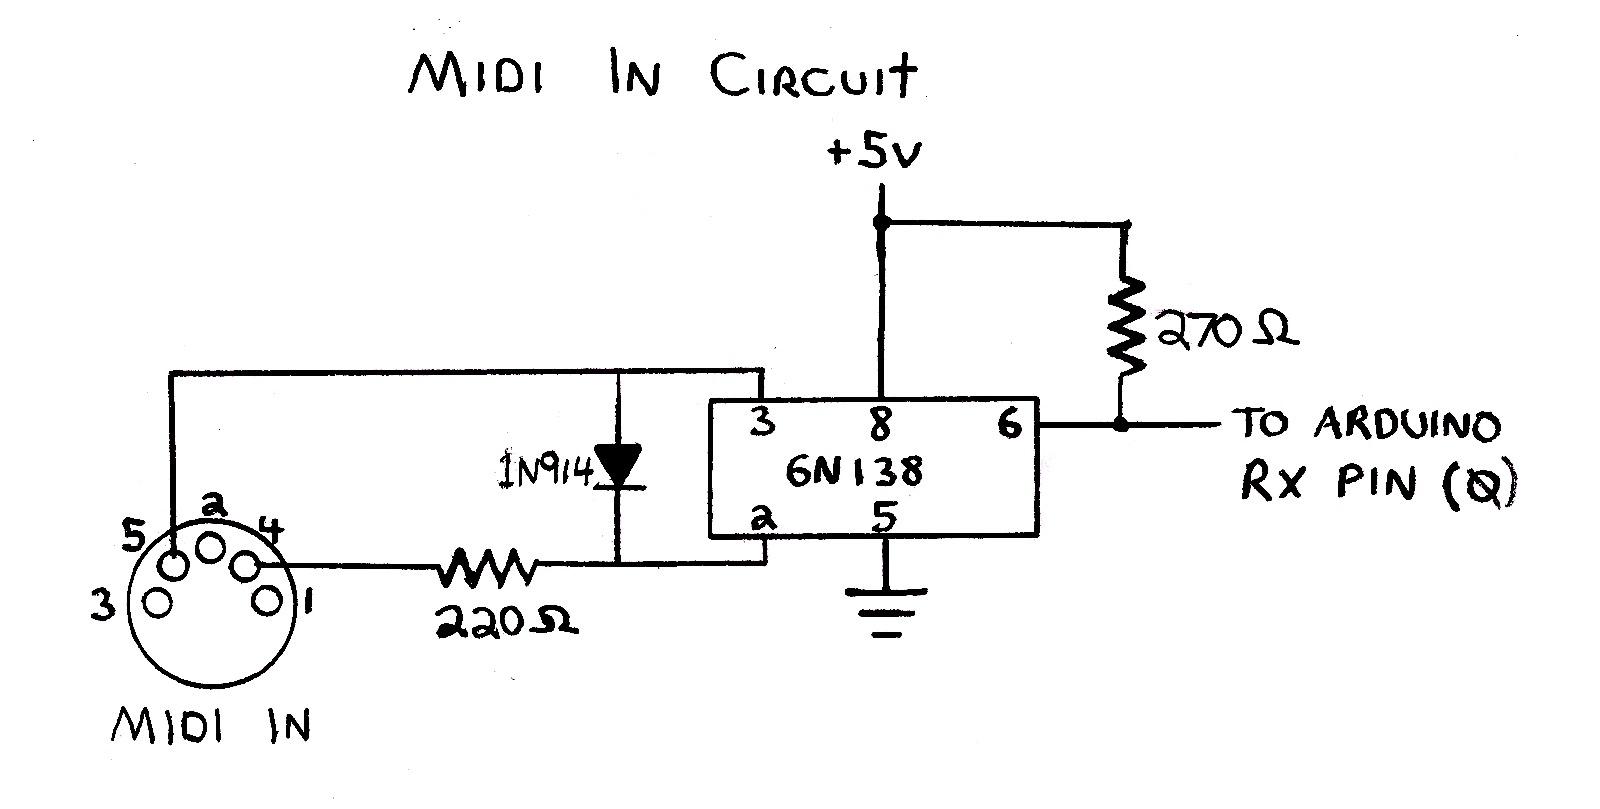
\includegraphics[width=0.36\textwidth]{graphics/arduino-midi-in}

\caption[
Arduino MIDI input circuit 
\newline 
\url{http://www.notesandvolts.com/2012/01/fun-with-arduino-midi-input-basics.html}]
{Arduino MIDI input circuit \label{fig-arduinocircuit}}

\end{center}
\vspace*{-2em} \end{wrapfigure}%
 This module is still at an experimental stage. The idea was to use
a digital microprocessor to be able to connect a keyboard to the synthesizer
and play it via MIDI. To achieve this the implementation of an Arduino
Uno was planned. Arduino is an open-source electronics prototyping
platform with a ATMega168 microprocessor at its heart. 

Conveniently the Arduino must be provided with a 9-12 volt power supply,
which made the process of connecting it to the synthesizers power
supply easy. Only the appropriate plug connection had to be put together.

The MIDI input communication has been established by the usage of
a 6N138 optocoupler, that isolates the Arduino circuit from the MIDI
device (see figure \ref{fig-arduinocircuit}). On the software side
the Arduino MIDI Library v3.2 has been included, which takes care
of interpreting the serial digital data arriving at the Arduino's
RX pin. 

What needs to be done next is converting the desired MIDI messages
into control voltages. The gate voltage would be easy to implement,
because it can be represented by a digital on/off state. The realization
of the pitch control voltage presents itself as more complex, since
the Arduino cannot output analog voltage values at its output pins
but only digital states. One way would be to create a high frequency
pulse width modulated signal and adding a low pass filter to convert
it to a stationary voltage. This may have the disadvantage of getting
a slight portamento effect though. The other way would be to convert
the possible 128 note values of the note on message into seven binary
values. These would be transmitted onto seven respective output pins.
A digital to analog converter (DAC) would then generate the analog
output voltage.

Regardless of which method is chosen, at the end the voltage should
be scaled to conform the 1 volt per octave interface.


\chapter{Conclusion}


\section*{Summary }

This paper is the result of a research on the topics of history, theory
and electronics of analog synthesis. Of course in all of the discussed
subjects only the surfaces could be scratched. Even only the field
of active filter circuitry can (and does) fill entire books. Accompanying
this research a small synthesizer prototype has been set up, making
use of the knowledge acquired during the research.


\section*{Results}

The objective to create a functional prototype can be considered a
complete success. The synthesizer that was built is a lot of fun to
experiment with, which was one of the initial goals also. Even though
it is practically just a self oscillating filter, it offers a lot
of possibilities for experimental sound design. Due to the fact that
the banana plugs are stackable, the two output signals can be split
several times to voltage control resonance and cutoff of each filter
stage. Also various types of feedback can be generated. 

This project provides a great basis for further sound experimentation.
Because of its modular setup, there is a lot of space for further
modules, although the requirements for power supply and case size
will increase with the number of modules. The next step will be the
construction of an oscillator module as soon as time and monetary
means allow it.


\section*{A Personal Journey}

As a trained programmer and web application developer the field of
electronic engineering always seemed appealing to me. Hence the assignment
for a research paper during the audio engineering course at SAE Institute
seemed like a welcome opportunity to dive into the realm of building
electronic devices in the context of sound generation and modification.

The process of writing this paper has been an unexpectedly rewarding
and inspiring experience, pushing the boundaries of my own musical
and technical understanding. Most notably the concepts of free composition
- meaning allowing randomness and therefore putting oneself in the
position of reacting to a musical system, influencing it in terms
of tendencies, rather than controlling it with a predetermined mindset
- has been something that really changed my perception of musical
creativity. This for me seems much more attainable in the analog world,
where electrical components and signal chains can be brought to their
tipping points, resulting in an unpredictable outcome. That is where
sound exploration begins, which is a totally different experience
than knowing what will happen. Virtual digital environments, which
I was familiar with on the other hand, generally seem to tend persuade
the user to feel in control at all times.


\section*{Acknowledgment}

At first I want to thank Fabian Gawlick and Sebastian Metzner for
introducing me to the topics of electronic engineering and sound synthesis.
I would like to thank Edmund Heineke Jaek for teaching me a lot about
amplification and helping me with the power supply for the prototype.
I am very grateful to Diego, Jano and Victor from befaco for their
awesome workshop and for helping me with a lot of tips and literature
on the discussed topics. A big thank you goes out to Derek Holzer,
who gave me an extended introduction into his self constructed modular
system and shared some valuable sound design concepts. Also I want
to thank Richard Pannek, David Markwart, Roosa Hämäläinnen and Vicki
Schmatolla for proof reading and their feedback on this paper. Lastly
I want to thank SAE institute for making this project possible.

\pagebreak


\chapter*{List of Figures}

{\makeatletter 
\let\@cftmakeloftitle\relax 
\listoffigures% Print List of Figures 
\makeatother}

\bibliographystyle{karl-second4}
\bibliography{synth_bibliography}



\chapter*{Declaration of academic honesty}

I hereby declare that in the attached submission I have not presented
anyone else’s work, in whole or in part, as my own using only the
admitted resources. Where I have taken advantage of the work of others,
I have given full acknowledgement.

\vspace{5em} 
\begin{tabular}{lp{2em}l}  
\hspace{5cm}   && 
\hspace{5cm} 
\\\cline{1-1}\cline{3-3}  Place, Date     && Signature \end{tabular}


\end{document}
